\thispagestyle{quantoannone}
\pagestyle{quantoan}
\everymath{\color{quantoan}}
\graphicspath{{../quantoan/pic/}}
%\blfootnote{\color{quantoan}\color{quantoan}$^*$Nguồn Math. Intellegencer, Số $41$.}
\begingroup
\AddToShipoutPicture*{\put(0,616){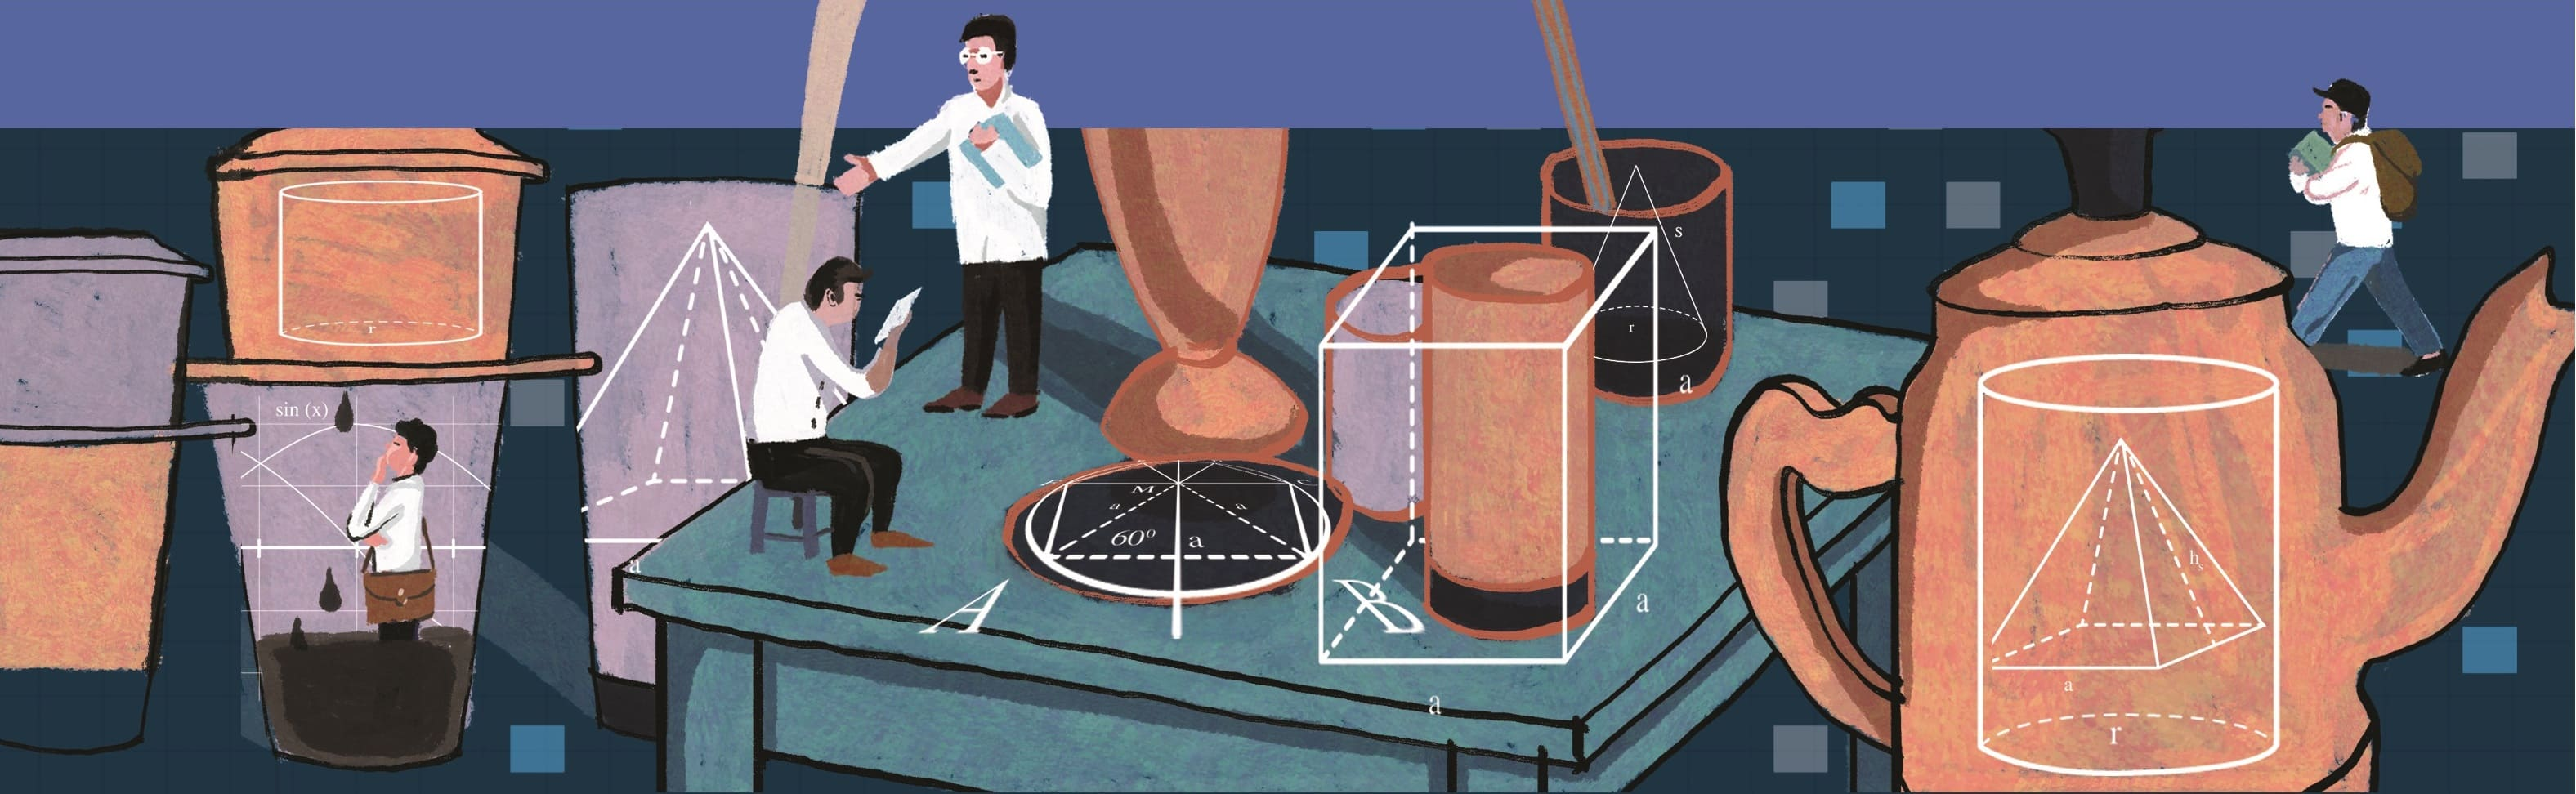
\includegraphics[width=19.3cm]{../bannerquantoan}}}
\AddToShipoutPicture*{\put(72,523){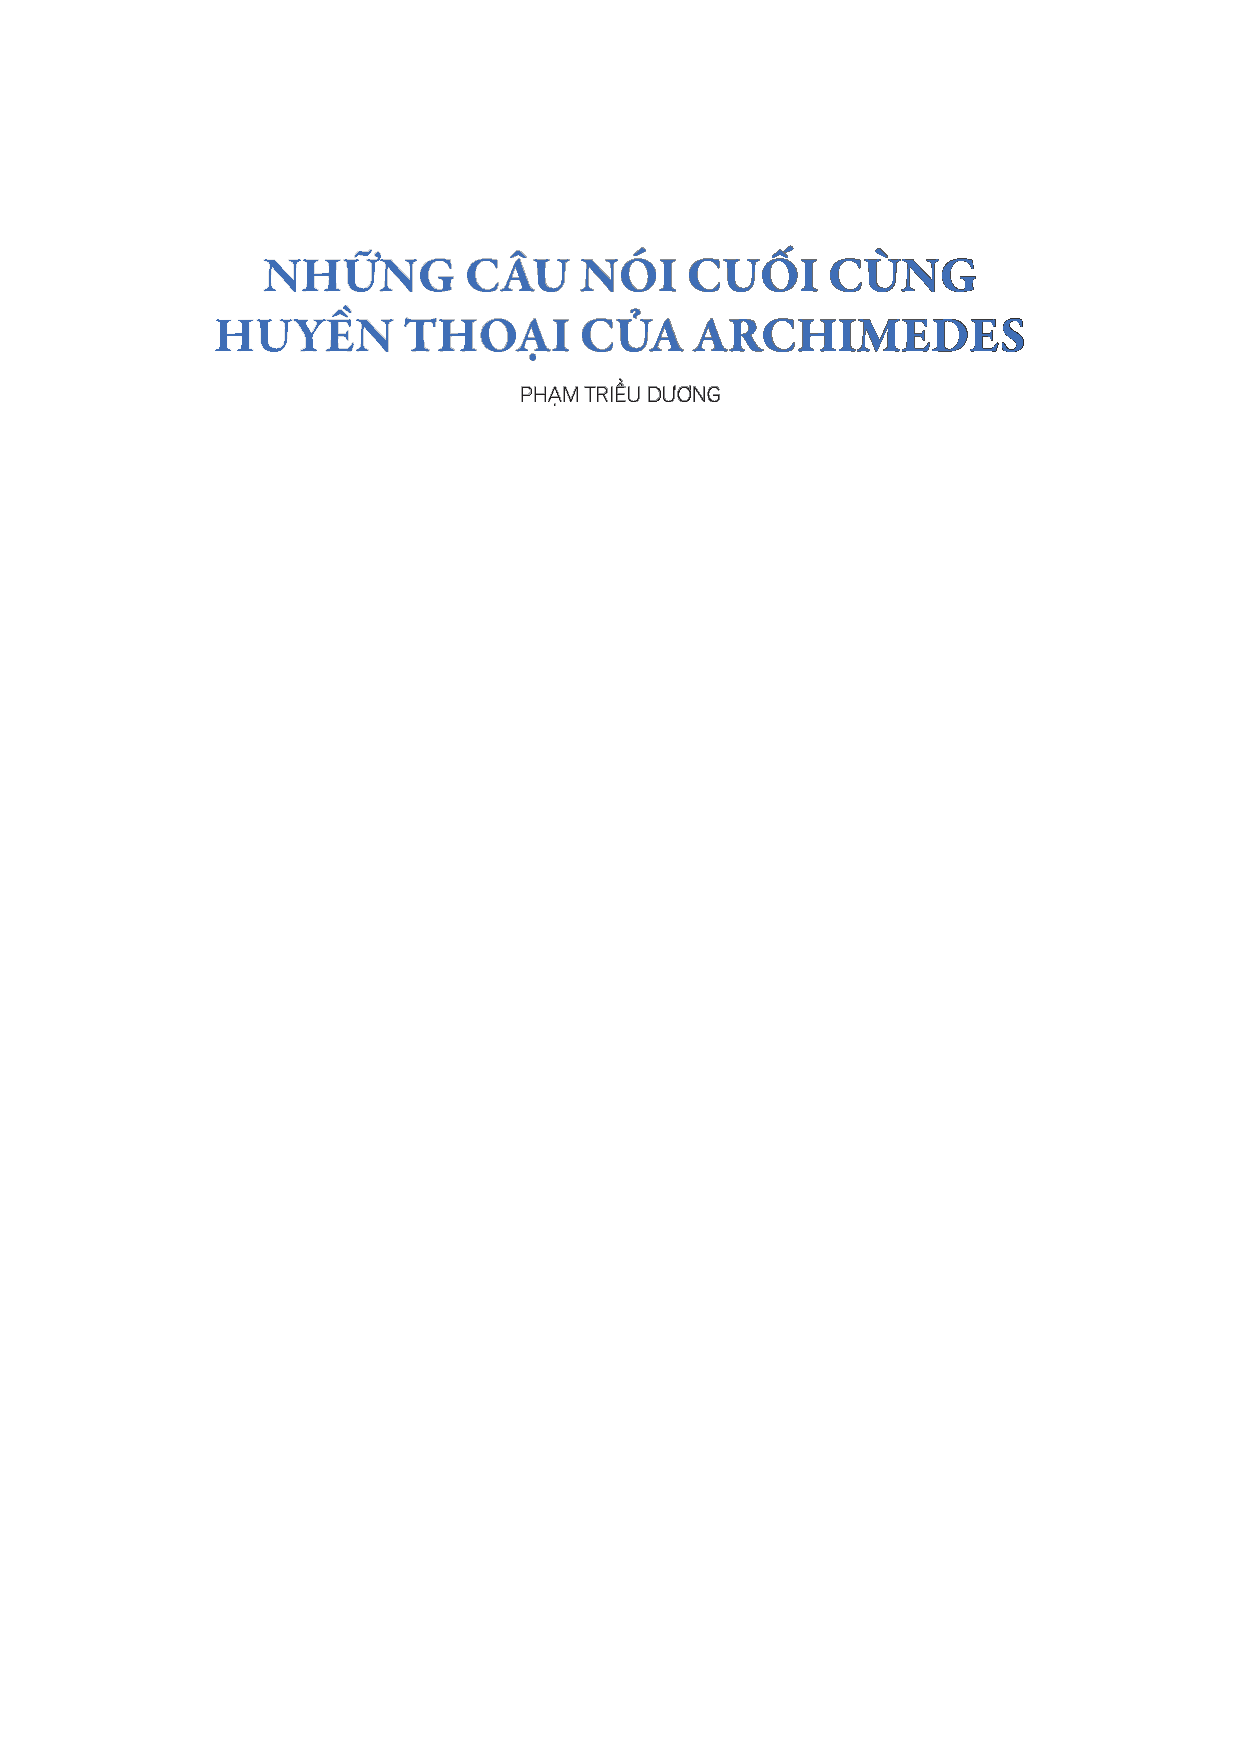
\includegraphics[scale=1]{../tieude1.pdf}}}
\centering
\endgroup
\vspace*{180pt}

\begin{multicols}{2}
	``\textit{Xin đừng xáo trộn những vòng tròn của tôi}"
	\vskip 0.1cm
	\hfill Μὴ μου τοὺς κύκλους τάραττε (tiếng Hy lạp)
	\vskip 0.1cm
	\hfill Noli turbare circulos meos (Tiếng La tinh)
	\vskip 0.1cm
	Khi chúng ta còn nhỏ, chắc hẳn ai cũng đều nghe tới chuyện về một ông già thời cổ đại nào đó, ông ta ngồi trên bờ biển, đang vẽ một cái hình gì đó trên cát thì một người lính cưỡi ngựa đi qua và đâm chiếc giáo làm ông già ngã xuống, ông ấy chỉ kịp thốt lên: ``Ôi, làm ơn đừng làm hỏng những hình vẽ của tôi".
	\begin{figure}[H]
		\vspace*{-5pt}
		\centering
		\captionsetup{labelformat= empty, justification=centering}
		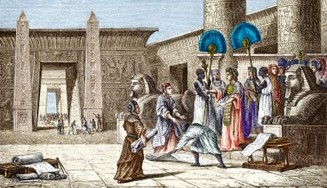
\includegraphics[width= 1\linewidth]{1}
%		\caption{\small\textit{\color{}}}
		\vspace*{-20pt}
	\end{figure}
	Câu chuyện này làm chúng ta mê say tới mức, lúc còn thơ ấu, cứ mỗi lần bạn và tôi đi nghỉ hè ở biển, chúng ta đều cố thử ngồi trên cát trắng và vẽ những hình tam giác, hình tròn và đợi những ngọn sóng ập tới xoá đi nhanh chóng những ký họa tạo ra trong những hình dung đẹp đẽ mơ hồ của chúng ta về một môn học gọi là Toán.
	\vskip 0.1cm
	Rồi tới khi học Vật lý, chúng ta lại được biết tới một ông già nào đó khác ở một xứ nọ, ông đang ngồi ngâm mình trong bồn tắm thì bỗng vùng dậy chạy ra đường và kêu lên: ``Eureka!" Tất cả các bạn bè của chúng ta đều yêu mến câu chuyện đó, và đều hay thốt lên một cách hồn nhiên ``Eureka!" khi muốn nói đến một khám phá bất chợt, giống như khi giải ra được một bài toán khó vào chiều tối thứ Sáu.
	\vskip 0.1cm
	Các câu chuyện trên đều về một người, đó là Archimedes xứ Syracuse ($287-212$). Về cái chết của ông, Wikipedia có viết ngắn gọn như sau: ``Archimedes chết trong đợt vây hãm thành Syracuse, ở đó ông bị một người lính La Mã giết mặc dù có mệnh lệnh phải bảo toàn tính mạng cho Archimedes." Vào lúc đó, Archimedes,  nổi tiếng với trí tuệ và kiến thức uyên thâm về hình học và cơ học, đã làm cho tướng quân La Mã là Marcus Claudius Marcellus phải nể phục. Marcellus biết rằng mình đã phải nhọc nhằn như thế nào trong việc chinh phục thành Syracuse cũng do các cỗ máy cơ học tinh xảo mà Archimedes chế tạo đã giúp dân thành chống cự được lính La Mã thiện chiến. Người La Mã nổi tiếng với tính tàn ác lạnh lùng, nhưng cũng là những người đề cao danh dự chiến trường. Vì quá hâm mộ tài năng xuất chúng của Archimedes, tướng quân Marcellus ra lệnh phải giữ mạng sống cho nhà toán học -- đối với Marcellus, cứu được Archimedes cũng đáng được coi là vinh quang như hạ được thành luỹ của Syracuse bằng gươm kiếm.
	\vskip 0.1cm
	Tuy nhiên, một người lính được cử đến để yêu cầu Archimedes nộp mình làm tù binh cho quân La Mã đã làm hỏng kế hoạch tỷ mỷ mà Marcellus nghĩ ra. Anh ta thô lỗ đạp cửa đột nhập vào nhà của Archimedes, đúng lúc  nhà toán học đang trầm ngâm mải mê vẽ những hình vẽ phức tạp. Người lính tuốt kiếm ra và hỏi Archimedes tên ông là gì. Archimedes, vì đang mải miết với công việc, không nhận thấy ai đang chỉ kiếm về mình, đã nói với người lính: ``Xin làm ơn đừng có làm xáo trộn những hình vẽ của tôi, anh bạn ơi!" Ông còn hét lên: ``Ai đưa giúp cho tôi một trong những cái máy của tôi nào!" Người lính La Mã, vì quá sợ hãi, theo bản năng tự vệ bèn đâm thẳng kiếm vào ông già yếu ớt, và cũng trong giây phút ấy đã hạ gục nhà toán học vĩ đại.
	\vskip 0.1cm
	Nhưng vì sao lại có câu chuyện về Archimedes bị đâm chết khi ngồi trên bãi cát nhỉ? Phần lớn các tài liệu đều đồng ý rằng ông đang ngồi tại nhà riêng và đang vẽ những hình hình học thì bị người lính đột nhập tới đâm ông bằng kiếm. Lúc đó Archimedes đang sử dụng một công cụ là bảng vẽ abax, một dụng cụ để vẽ bằng bụi cát. Vì vậy mới có dị bản trên về bãi cát như tôi và các bạn đã từng nghe khi còn nhỏ.
	\begin{figure}[H]
		\vspace*{-5pt}
		\centering
		\captionsetup{labelformat= empty, justification=centering}
		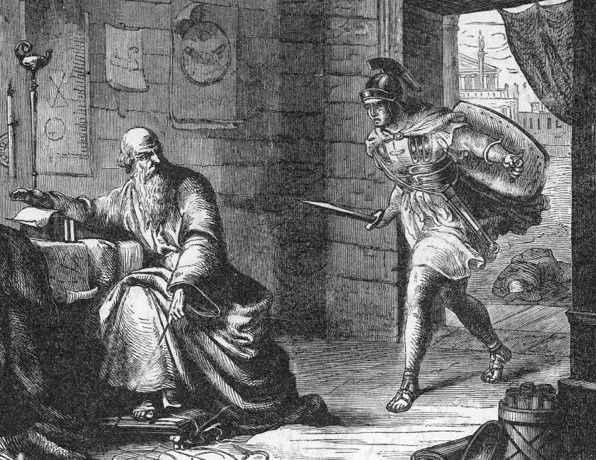
\includegraphics[width= 1\linewidth]{2}
%		\caption{\small\textit{\color{}}}
		\vspace*{-15pt}
	\end{figure}
	Ân hận với hành động bất cẩn của quân lính, Marcellus đã xin lỗi họ hàng của Archimedes và cho đặt trên mộ của ông một biểu tượng mô tả một hình cầu đặt trong một hình trụ, và mãi $137$ năm sau, một chính trị gia La Mã là Cicero mới tìm thấy ngôi mộ này của nhà toán học. Người La Mã cổ đại nói chung không quan tâm tới toán học, và hành động dọn dẹp ngôi mộ cho phong quang của Cicero có lẽ là đóng góp đáng ghi nhớ nhất của bất kỳ người La Mã nào đối với lịch sử phát triển của toán học.
	\begin{figure}[H]
		\vspace*{-5pt}
		\centering
		\captionsetup{labelformat= empty, justification=centering}
		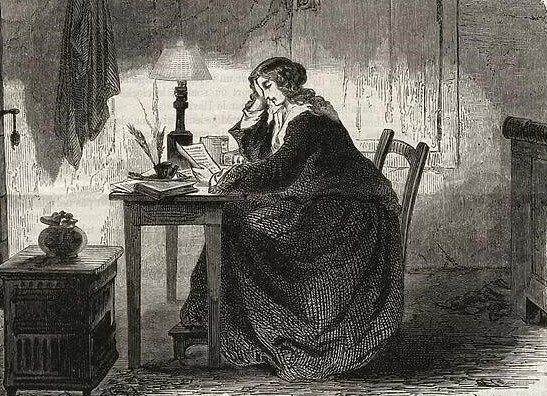
\includegraphics[width= 1\linewidth]{4}
		\caption{\small\textit{\color{quantoan}Sophie Germain ($1776-1831$) -- Nhà toán học, vật lý học và triết học người Pháp.}}
		\vspace*{-10pt}
	\end{figure}
	Sự thiên tài và đầu óc luôn muốn tò mò khám phá tri thức của Archimedes tiếp tục truyền cảm hứng tới nhiều nhà tư tưởng khác rất lâu sau khi ông qua đời, từ Galileo cho tới Issac Newton. Chúng ta có thể nhắc tới Sophie Germain, một nhà toán học nữ người Pháp sinh năm $1776$. Vào năm $13$ tuổi, cô đã được đọc câu chuyện về cái chết của Archimedes. Sophie cho rằng bất kỳ môn học nào mà có thể thu hút một người tập trung say mê như vậy đều đáng để nghiên cứu, và cô quyết định tự học toán -- đặc biệt là môn lý thuyết số. Cha mẹ cô đã lo lắng rất nhiều về sở thích toán học của con gái mình khi cô còn là một cô bé, và vào thời cô sống, việc phụ nữ trở thành một nhà toán học là điều không bình thường, vì vậy họ đã tịch thu tất cả các cây nến của cô và dỡ bỏ mọi thiết bị sưởi ấm trong phòng cô. Cô đáp lại bằng cách bí mật thắp nến rồi ngồi vào bàn, quấn chăn kín người. Cha mẹ cô cuối cùng đã mủi lòng và quyết định tài trợ cho việc học hành của cô. Sophie, sau khi tìm thấy một sinh viên sắp rời Paris tên là Antoine--August Le Blanc, đã bí mật thế chỗ anh ta, sử dụng tên của anh ta để gửi và nhận tài liệu từ École Polytechnique khi đó mới mở,  vì trường chỉ nhận sinh viên nam tới học. Joseph--Louis Lagrange, lúc đó là người hướng dẫn của Sophie, đã rất ngạc nhiên khi  sinh viên này có thể tiến bộ rất nhiều -- từ một học sinh tệ hại trở thành người có bài tập giải hàng tuần (tất nhiên là được gửi qua đường bưu điện) là tốt nhất trong lớp. Lagrange yêu cầu được gặp ``anh" sinh viên Le Blanc và ngạc nhiên khi biết rằng ``anh ta" hoá ra là một quý cô! Sophie đã trở thành một trong những nhà lý thuyết số xuất chúng nhất trong thời đại của cô.
	\vskip 0.1cm
	Chắc các bạn đọc đến đây đã yêu thích hơn chiếc bàn học ngăn nắp của mình được rọi chiếu bởi ánh sáng thoáng đãng rồi chứ?
	\vskip 0.1cm
	Tham khảo dựa trên các nguồn internet:
	\vskip 0.1cm
	[$1$]	\url{https://math.nyu.edu/~crorres/Archim} \linebreak\url{edes/contents.html}
	\vskip 0.1cm
	[$2$]	\url{https://en.wikipedia.org/w/index.php?title=Archimedes&oldid=1146936468}
\end{multicols}
\vspace*{-10pt}
{\color{quantoan}\rule{1\linewidth}{0.1pt}}
\begingroup
\AddToShipoutPicture*{\put(130,458){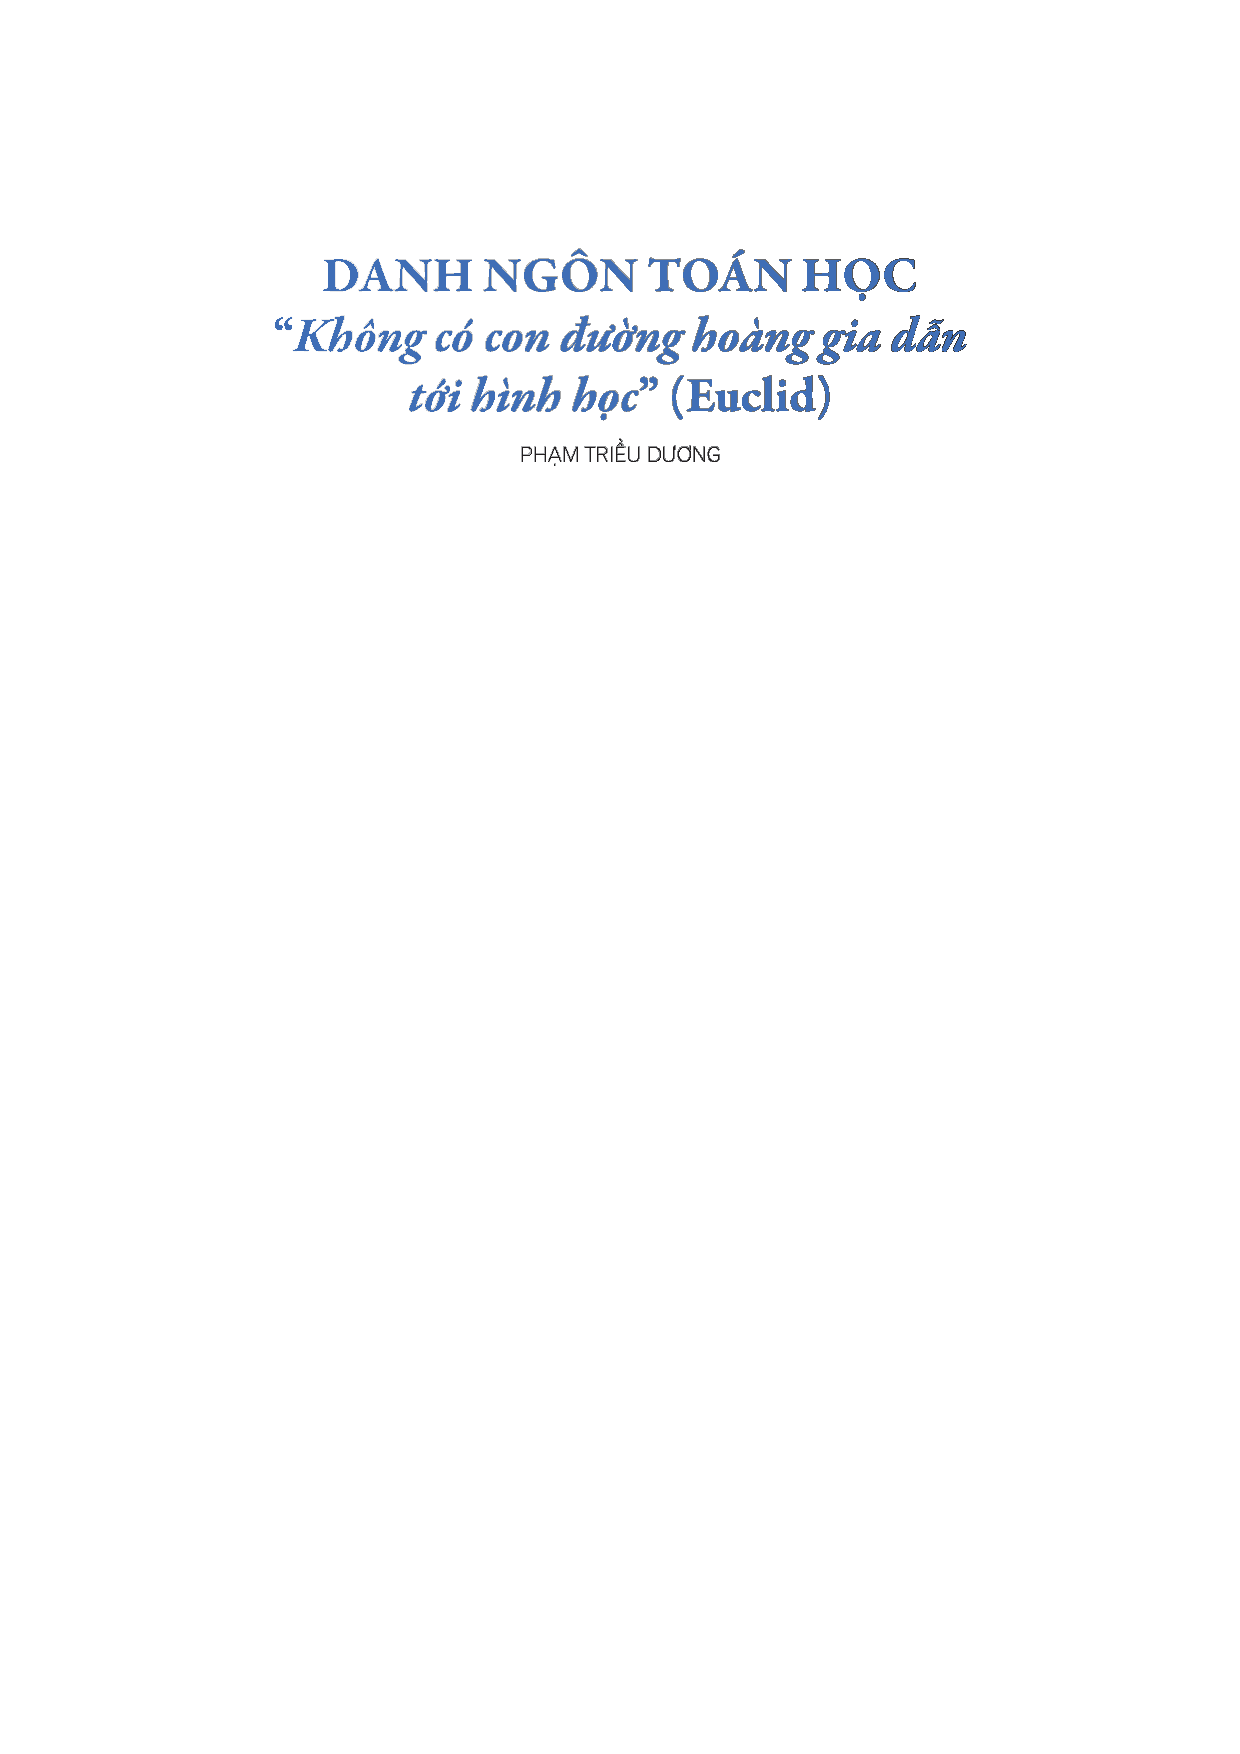
\includegraphics[scale=1]{../tieude.pdf}}}
\centering
\endgroup
\vspace*{40pt}

\begin{multicols}{2}
	Trò chơi ``Tháp Hà Nội", xếp những miếng gỗ trên ba chiếc cọc, đã rất quen thuộc với các bạn nhỏ Việt Nam cũng như nhiều bạn nhỏ trên thế giới. Thật là tuyệt vời khi một trò chơi nổi tiếng trên thế giới lại có tên liên quan đến thủ đô của nước ta đúng không. Các bạn đã biết về xuất xứ cùng với nhiều điều thú vị xung quanh bài toán ``Tháp Hà Nội" chưa? Chúng ta hãy cùng ngược dòng thời gian để tìm hiểu qua bài viết dưới đây nhé.
	\begin{figure}[H]
		\centering
		\vspace*{-5pt}
		\captionsetup{labelformat= empty, justification=centering}
		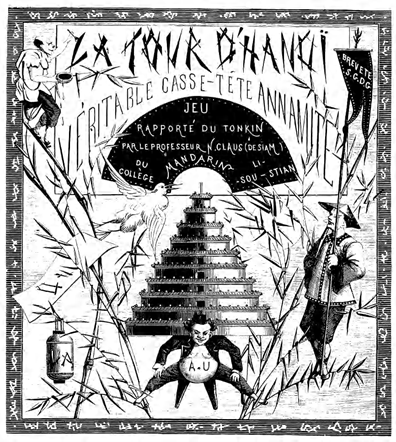
\includegraphics[width=1\linewidth]{1.1}
		%	\caption{\textit{\color{toancuabi}Hình $1$.}}
		\vspace*{-15pt}
	\end{figure}
	Năm $1883$, Eduard Lucas (Claus) công bố  bức tranh quảng cáo ``Tháp Hà Nội --  trò chơi thực sự nát óc xứ Annnam".
	\vskip 0.1cm
	Một năm sau, Lucas viết bài ``Tháp Hà Nội , trò chơi toán học" đăng ở tạp chí ``Science et Nature", số $1$ ($1884$) tr. $127-128$. Có thể xem đó ngày khai sinh của ``Bài toán Tháp Hà Nội", một trong những bài toán nổi tiếng của toán học. Cho đến ngày nay, vẫn còn rất nhiều công trình nghiên cứu về bài toán tháp Hà Nội và những mở rộng của nó, vẫn còn nhiều giả thuyết đang chờ câu trả lời.
	\vskip 0.1cm
	Hình sau đây là bức ảnh chụp từ hiện vật trưng bày trong ``Musée des arts et métiers--Cnam Paris" (Bảo tàng nghệ thuật và thủ công Paris). 
	\vskip 0.1cm
	Ta có ba cái cọc, và  $8$ cái đĩa với kích thước khác nhau đôi một. Bài toán đặt ra là di chuyển toàn bộ $8$ cái đĩa sang một cọc khác, sao cho vẫn giữ được thứ tự các đĩa với bán kính lớn dần từ trên xuống dưới. Quy tắc di chuyển: mỗi lần chỉ được chuyển một đĩa, và không bao giờ được đặt một đĩa lên đĩa khác có bán kính nhỏ hơn. Điều này có thể làm được nhờ sử dụng cọc ``trung gian".
	\begin{figure}[H]
		\centering
		\vspace*{5pt}
		\captionsetup{labelformat= empty, justification=centering}
		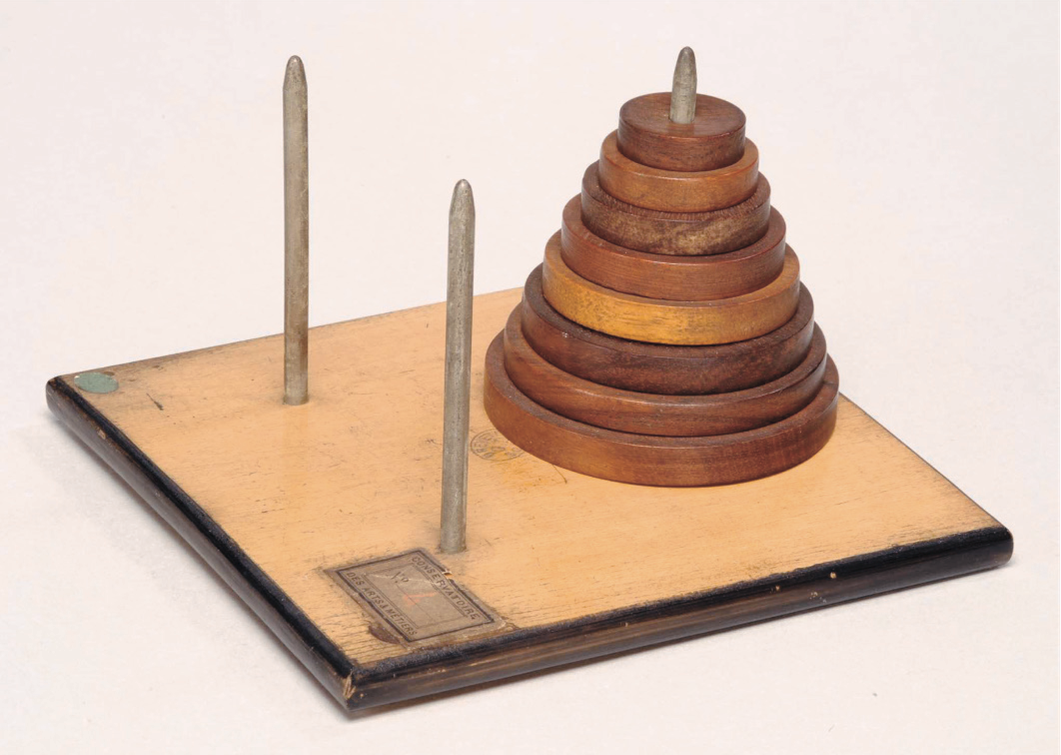
\includegraphics[width=1\linewidth]{2.1}
		%	\caption{\textit{\color{toancuabi}Hình $1$.}}
		\vspace*{-15pt} 
	\end{figure}
	Các bạn thử hình dung xem ta sẽ cần làm bao nhiêu phép chuyển đĩa?
	\vskip 0.1cm
	Trước hết, ta thử làm bài toán dễ hơn: trên cọc chỉ có $2$ đĩa. Rõ ràng chỉ cần chuyển đĩa nhỏ sang cọc trung gian, đĩa lớn sang cọc còn lại, rồi chuyển đĩa nhỏ lên cọc đó. Số bước chuyển là $3$.
	\vskip 0.1cm
	Nếu có $3$ đĩa trên cọc thì sao? Giả sử các đĩa đang ở cọc $A$, và ta cần chuyển sang cọc $C$. Ta chuyển hai đĩa trên cùng sang cọc  trung gian $B$, rồi chuyển đĩa to nhất sang cọc $C$. Sau đó chỉ cần chuyển hai đĩa từ cọc $B$ sang cọc $C$. Phương pháp chuyển $2$ đĩa từ cọc này sang cọc khác thì ta đã biết. Như vậy, số phép chuyển phải làm khi có $3$ đĩa bằng $2$ lần số phép chuyên khi có $2$ đĩa, cộng thêm $1$ phép chuyển (đĩa to nhất). 
	\vskip 0.1cm
	Như vậy, số bước chuyển cần thiết của $3$ đĩa là: $2\times 3 + 1 = 7$. Bằng quy nạp, dễ chứng minh nếu $N$ là số phép chuyển khi có $n$ đĩa thì với $(n+1)$ đĩa, ta có thể thực hiện nhiệm vụ với $(2N+1)$ phép chuyển. Từ đó, dễ suy ra, nhiệm vụ đặt ra trong bài toán Tháp Hà Nội với $n$ đĩa có thể thực hiện với $2^n- 1$  phép chuyển.
	\vskip 0.1cm
	Có thể chứng minh $2^n - 1$  là số phép dịch chuyển tối thiểu cần thiết, nghĩa là không có cách gì thực hiện nhiệm vụ với số phép dịch chuyển ít hơn.
	\vskip 0.1cm
	Người ta cho rằng, bài toán Tháp Hà Nội lấy ý tưởng từ câu chuyển cổ Ấn Độ sau đây.
	\vskip 0.1cm
	``Trong ngôi đền vĩ đại ở Benares, bên dưới mái vòm đánh dấu trung tâm thế giới, người ta đặt một chiếc đĩa bằng đồng, trên đó gắn cố định ba chiếc cọc kim cương, mỗi chiếc cao một mét và dày như thân của một con ong. Trên một trong những chiếc cọc  kim cương đó, vào buổi sáng tạo, Thượng Đế đặt $64$ chiếc đĩa bằng vàng nguyên chất, theo thứ tự to dần từ trên xuống dưới.  Ngày đêm không ngừng, những con quỷ chuyển các đĩa từ cọc kim cương này sang cọc kim cương khác theo nguyên tắc không được di chuyển nhiều hơn một đĩa cùng một lúc, và không được đặt đĩa nào lên trên cái nhỏ hơn nó. Khi $64$ chiếc  đĩa  được chuyển xong thì tiếng sét sẽ nổ ra, và thế giới tan biến".
	\vskip 0.1cm
	Những suy luận trên đây chỉ ra rằng, số phép dịch chuyển mà lũ quỷ phải làm ít nhất là
	\begin{align*}
		2^{64} - 1= 18{.}446{.}744{.}073{.}709{.}551{.}615.
	\end{align*}
	Giả sử lũ quỷ rất thạo ``thuật toán dịch chuyển", và mỗi giây chúng chuyển được một đĩa, thì phải mất khoảng $585$ tỷ năm. Có lẽ dù không có lũ quỷ, trái đất của chúng ta cũng không tồn tại được lâu đến thế!
	\vskip 0.1cm
	Từ sau khi ra đời, bài toán Tháp Hà Nội nhận được sự quan tâm lớn của các nhà toán học và những người làm ... đồ chơi. Rất nhiều phiên bản của bài toán Tháp Hà Nội xuất hiện, chẳng hạn như số cọc lớn hơn $3$, hoặc cách chơi có thay đổi. Cho đến ngày nay, Tháp Hà Nội và những biến thể của nó vẫn là bài toán quan trọng trong toán học rời rạc, lý thuyết đồ thị, khoa học máy tính, và tô pô (chẳng hạn, bài toán về đường cong tự cắt tại mọi điểm của nó!). Thậm chí, Tháp Hà Nội còn có ứng dụng rộng rãi trong nghiên cứu tâm lý học!
	\vskip 0.1cm
	Người ta cho rằng, sở dĩ bài toán Tháp Hà Nội lôi cuốn được nhiều thế hệ các nhà toán học vì nó chứa đựng những yếu tố làm nên sức hấp dẫn của Toán học: đẹp, thú vị, hữu ích, và bất ngờ.
\end{multicols}
\newpage
\begingroup
\blfootnote{$^1$\color{quantoan}Mathematics as an adequate language.}
\AddToShipoutPicture*{\put(106,677){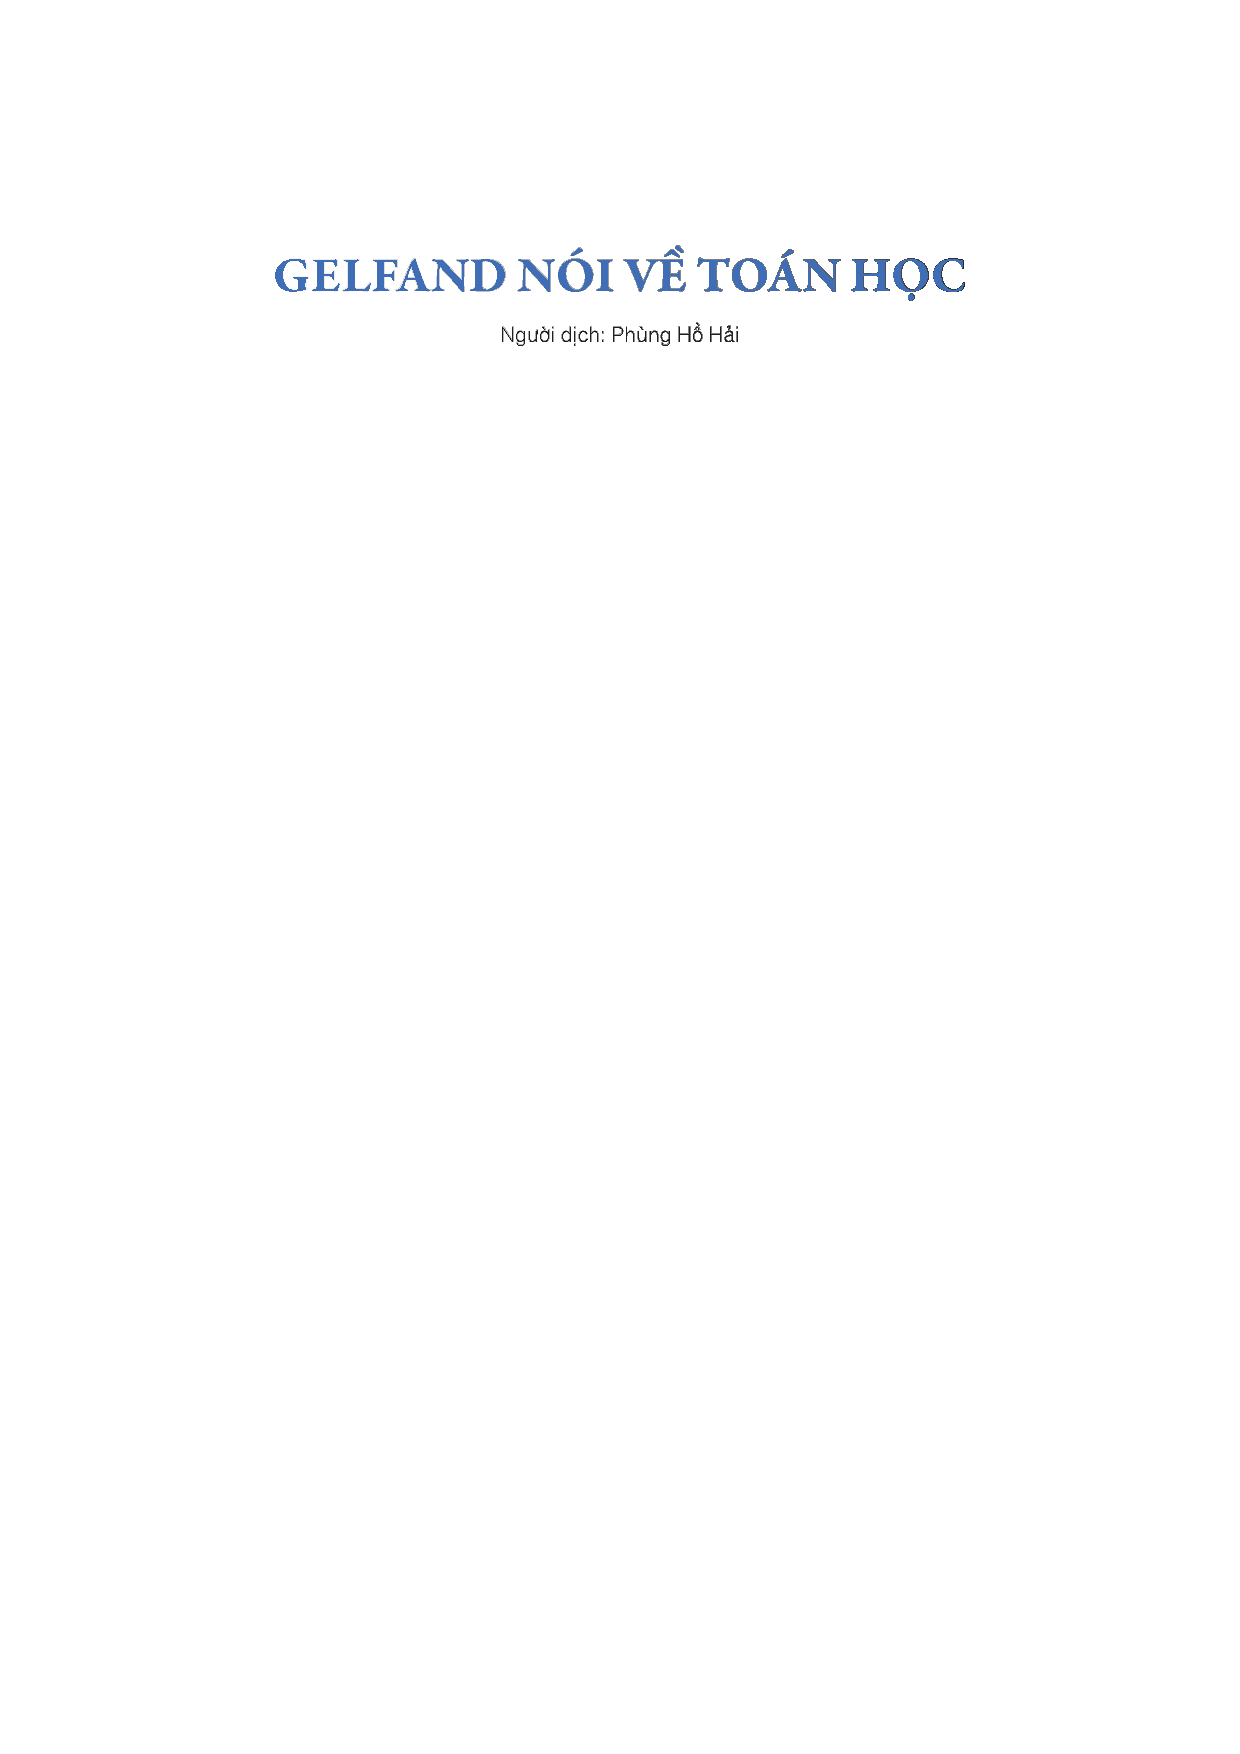
\includegraphics[scale=1]{../tieude3.pdf}}}
\centering
\endgroup
\vspace*{40pt}

\textit{\textbf{\color{quantoan}Lời người dịch.} Israel M. Gelfand $(1913-2009)$ là một trong những nhà toán học vĩ đại nhất của thế kỷ XX. Năm $2003$, các đồng nghiệp và học trò ông đã tổ chức một hội thảo khoa học lớn tại Đại học Harvard để kỷ niệm $90$ năm ngày sinh của ông. Bản thân Gelfand cũng trình bày báo cáo với tiêu đề ``Toán học như một ngôn ngữ phù hợp"$^1$. Các báo cáo tại hội thảo về sau được xuất bản thành cuốn sách ``Sự  thống nhất của Toán học" (The unity of Mathematics). Bài viết giới thiệu những chia sẻ của Gelfand tại hội thảo. Các tiêu đề do người dịch đặt.}
\begin{multicols}{2}
	\begin{figure}[H]
		\vspace*{5pt}
		\centering
		\captionsetup{labelformat= empty, justification=centering}
		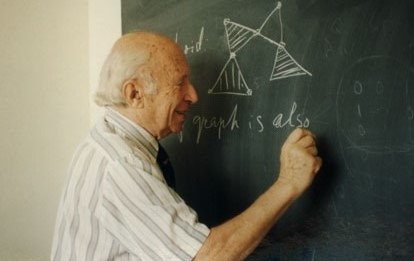
\includegraphics[width= 1\linewidth]{gelfand_blackboard}
%		\caption{\small\textit{\color{}.}}
		\vspace*{-20pt}
	\end{figure}
	\textbf{\color{quantoan}Toán học là gì?}
	\vskip 0.1cm
	Theo quan điểm của tôi, toán học là một phần của nền văn hóa của chúng ta, giống như âm nhạc, thơ ca và triết học. Tôi đã nói về điều này trong bài giảng của tôi tại hội thảo. Ở đó, tôi đã đề cập đến sự gần gũi giữa phong cách toán học và phong cách âm nhạc cổ điển hay thơ ca. Tôi rất vui khi tìm thấy bốn đặc điểm chung sau: thứ nhất, vẻ đẹp; thứ hai, sự đơn giản; thứ ba, tính chính xác; thứ tư, những ý tưởng điên rồ. Sự kết hợp của bốn điều này: vẻ đẹp, tính chính xác, sự đơn giản và những ý tưởng điên rồ chính là trái tim của toán học, trái tim của âm nhạc cổ điển. Nhạc cổ điển không chỉ là nhạc của Mozart, hay Bach, hay Beethoven. Nó cũng là nhạc của Shostakovich, Schnittke, Schoenberg (nhạc của người cuối cùng tôi hiểu ít hơn). Tất cả đó là âm nhạc cổ điển. Và tôi nghĩ rằng cả bốn đặc điểm này luôn hiện hữu trong đó. Vì lý do này, không phải ngẫu nhiên mà các nhà toán học lại thích nhạc cổ điển. Họ thích nó vì nó có cùng phong cách tổ chức tâm lý.
	\vskip 0.1cm
	Ngoài ra còn có một khía cạnh khác của sự tương đồng giữa toán học và âm nhạc cổ điển, thơ ca, v.v. Đây là những ngôn ngữ để hiểu nhiều thứ. Ví dụ: Tại sao các nhà triết học Hy Lạp vĩ đại lại nghiên cứu hình học? Họ là những triết gia. Họ đã học hình học như triết học. Các nhà hình học vĩ đại đã đi theo và làm theo cùng một truyền thống để thu hẹp khoảng cách giữa viễn kiến và lập luận. Chẳng hạn các tác phẩm của Euclid đã tóm tắt khuynh hướng này trong thời\linebreak của ông.  
	\vskip 0.1cm
	\textbf{\color{quantoan}Toán học như một ngôn ngữ phù hợp}
	\vskip 0.1cm
	Một khía cạnh quan trọng của toán học là nó là một ngôn ngữ phù hợp cho các lĩnh vực khác nhau: vật lý, kỹ thuật, sinh học. Ở đây, cụm từ quan trọng nhất là ``ngôn ngữ phù hợp". Chúng ta có ngôn ngữ phù hợp và không phù hợp. Tôi có thể cung cấp cho bạn các ví dụ về ngôn ngữ phù hợp và không phù hợp. Ví dụ, [sử dụng] cơ học lượng tử trong sinh học không phải là ngôn ngữ phù hợp, nhưng [sử dụng] toán học trong nghiên cứu trình tự gen là ngôn ngữ phù hợp.  
	\vskip 0.1cm
	Tại sao đây là vấn đề quan trọng vào lúc này? Nó quan trọng bởi vì chúng ta đang có một cuộc ``cái tổ" trong thời đại này. Chúng ta có máy tính có thể làm mọi thứ. Chúng ta không bị ràng buộc bởi các phép tính cộng và nhân. Chúng ta cũng có rất nhiều công cụ. Tôi chắc chắn rằng trong $10$ đến $15$ năm nữa, toán học sẽ hoàn toàn khác so với trước đây.
	\vskip 0.1cm
	\textbf{\color{quantoan}Làm sao tôi có thể làm toán ở tuổi chín mươi?}
	\vskip 0.05cm
	Câu trả lời rất đơn giản. Tôi không phải là một nhà toán học vĩ đại. Tôi nói nghiêm túc. Tôi chỉ là một học sinh trong suốt cuộc đời của tôi. Ngay từ khi bắt đầu cuộc đời, tôi đã cố gắng học hỏi. Và ví dụ như bây giờ, khi nghe các báo cáo và đọc các bản thảo ở hội nghị này, tôi phát hiện ra rằng mình còn nhiều điều chưa biết và phải học hỏi. Vì vậy, tôi luôn luôn học hỏi. Theo nghĩa này, tôi là một học sinh -- không bao giờ là một \linebreak ``Lãnh tụ."
	\vskip 0.05cm
	Tôi muốn nhắc đến những người thầy của tôi. Tôi không thể kể những ai là thầy của tôi là ai vì có quá nhiều người. Khi tôi còn trẻ, khoảng $15-16$ tuổi, tôi bắt đầu học toán. Tôi không được học hành chính quy, tôi chưa bao giờ tốt nghiệp đại học, tôi ``nhảy" qua bậc này. Năm $19$ tuổi, tôi trở thành nghiên cứu sinh và tôi học hỏi từ những đồng nghiệp lớn tuổi hơn.
	\vskip 0.05cm
	Vào thời điểm đó, một trong những người thầy quan trọng nhất đối với tôi là Schnirelmann, một nhà toán học thiên tài, qua đời khi còn trẻ. Sau đó là Kolmogorov, Lavrentiev, Plesner, Petrovsky, Pontryagin, Vinogradov, Lusternik. Tất cả đều khác nhau. Tôi thích một số người trong họ và tôi hiểu một số trong họ giỏi như thế nào nhưng tôi không tán thành -- nói một cách nhẹ nhàng là vậy -- quan điểm của họ. Nhưng họ là những nhà toán học vĩ đại. Tôi rất biết ơn tất cả họ, và tôi đã học được rất nhiều điều từ họ.
	\vskip 0.05cm
	\textbf{\color{quantoan}Sự thống nhất của toán học}
	\vskip 0.05cm
	Khi chúng ta nghĩ về âm nhạc, chúng ta không phân chia nó thành những lĩnh vực cụ thể như chúng ta thường làm trong toán học. Nếu chúng ta hỏi một nhà soạn nhạc nghề nghiệp của anh ta là gì, anh ta sẽ trả lời, ``Tôi là một nhà soạn nhạc." Khó mà có chuyện anh trả lời, "Tôi là một nhà soạn nhạc cho tứ tấu." Có lẽ đây là lý do tại sao, khi tôi được hỏi nghiên cứu lĩnh vực nào của toán học, tôi chỉ trả lời, ``Tôi là một nhà toán học."
	\vskip 0.03cm
	Tôi may mắn được gặp Paul Dirac vĩ đại, người mà tôi đã ở cùng vài ngày ở Hungary. Tôi học được nhiều thứ từ ông ấy.
	\vskip 0.03cm
	Vào những năm $1930$, nhà vật lý trẻ Pauli đã viết một trong những cuốn sách hay nhất về cơ học lượng tử. Trong chương cuối của cuốn sách này, Pauli thảo luận về các phương trình Dirac. Ông viết rằng các phương trình Dirac có những điểm yếu bởi vì chúng đưa ra những kết luận khó xảy ra và thậm chí \linebreak điên rồ:
	\vskip 0.03cm
	$1.$	Các phương trình này giả định rằng, bên cạnh electron, còn tồn tại một hạt mang điện tích dương, positron, mà chưa ai từng quan sát thấy.
	\vskip 0.03cm
	$2.$	Hơn nữa, electron hành xử một cách kỳ lạ khi gặp positron. Cả hai triệt tiêu lẫn nhau và tạo thành hai photon.
	\vskip 0.03cm
	Và điều hoàn toàn điên rồ là:
	\vskip 0.03cm
	$3.$	Hai photon có thể biến thành một cặp electron--positron.
	\vskip 0.03cm
	Pauli viết rằng mặc dù vậy, các phương trình Dirac khá thú vị và đặc biệt là các ma trận Dirac đáng được quan tâm.
	\vskip 0.03cm
	Tôi hỏi Dirac, ``Paul, tại sao, bất chấp những nhận xét này, anh không từ bỏ các phương trình của mình mà tiếp tục theo đuổi các kết quả của mình?"
	\vskip 0.03cm
	``Bởi vì, chúng đẹp."
	\vskip 0.03cm
	Bây giờ là lúc cho một cuộc cải tổ triệt để ngôn ngữ cơ bản của toán học. Lúc này, điều đặc biệt quan trọng là phải ghi nhớ sự thống nhất của toán học, ghi nhớ vẻ đẹp, sự đơn giản, tính chính xác và những ý tưởng điên rồ của nó. Tôi muốn nhắc lại rằng khi phong cách âm nhạc thay đổi vào thế kỷ $20$, nhiều người nói rằng âm nhạc hiện đại thiếu sự hài hòa, không tuân theo các quy tắc chuẩn mực, nghịch tai, v.v. Tuy nhiên, âm nhạc của Schoenberg, Stravinsky, Shostakovich và Schnittke cũng chính xác như âm nhạc của Bach, Mozart và Beethoven trước đây.
\end{multicols}